\chapter{Opis projektnog zadatka}
		
		%\textbf{\textit{dio 1. revizije}}\\
		
		\textit{Cilj projekta „Djeca za djecu“ je razviti web aplikaciju koja će omogućiti roditeljima, i onim budućim, da lakše doniraju i pronalaze donacije za svoju djecu. }\\
		\textit{U doba kada su već osnovne namirnice preskupe i globalno zagađenje raste, „recikliranje“ predmeta postaje još važnije. Zašto bacati dobro očuvane stvari koje još mogu poslužiti nekome i spasiti njegov džep, a nemamo ih gdje čuvati dok ne zatrebaju kolegi/prijateljima/rodbini…  }\\
		\newline
		\textit{Ova aplikacija brzo i efikasno spaja donatora i primatelja donacije bez da korisnici moraju pretraživati bespuća interneta. Oglasi u aplikaciji prilagođavaju se profilu korisnika. Nakon što korisnik jednom upiše svoje podatke i podatke o svojoj djeci korisniku se automatski prikazuju oglasi od interesa. Dodatno se mogu namještati filteri kategorija kod pregleda oglasa. }\\
		\textit{Doniranje, također, nikada nije bilo lakše. Nakon što korisnik objavi oglas za predmet više se ne mora brinuti o njemu dok aplikacija sama ne pronađe savršenog primatelja. Tek kada predmet pronađe svog potencijalnog novog vlasnika zamišljeno je da se primatelj kontaktira donatora izvan aplikacije te se dogovori za primopredaju. \color{red} Nakon izvršene donacije donator treba samo potvrditi da je donirao korisniku upisivanjem korisničkog imena primatelja.}\\
		\newline
		\textit{Sigurnost i kredibilitet aplikacije i oglasa je važan za iskustvo korisnika. Stoga je aplikacija zatvorena na registrirane korisnike što omogućava praćenje aktivnosti unutar aplikacije. Provode se provjere na razini korisnika i oglasa. Korisnici \color{red}(ADMIN van aplikacije) \color{black}se provjeravaju na temelju prijašnjih donacija ili postojećih zapisa o njima kako bi eliminirali moguće prevare ostalih korisnika aplikacije. Oglasi, pak, moraju biti opisani u skladu sa standardom aplikacije i \color{red}predmeti ne stariji od preporučene starosti za određen predmet. }
		\newline

		\textit{Istraživanjem hrvatskog „tržišta“ za sličnim aplikacijama pokazalo je da ne postoje aktivne aplikacije za doniranje i razmjenu dječjih stvari. U 2017. godini govorilo se o BIPO CLUB aplikaciji (poznatog BIPO branda za djecu, trgovačkog lanca BIPA) za razmjenu dječjih stvari koja trenutno više nije dostupna. Kako su odgovorili iz BIPO kluba aplikacija se ne koristi te su gašenjem iste spojili BIPO i BIPA kartice te se ne može više aktivirati korisnički račun u aplikaciji..}
		\begin{figure}[h!]
			\center
			
\includegraphics[width = \linewidth]{Picture1.png}
			\caption{Objavljena na \url{https://supermame.hr/2017/07/07/nova-mobilna-aplikacija-bipo-klub-razmjenu-djecjih-stvari-opreme/}}
			\label{fig1}
		\end{figure}
		\newline
		\textit{Za razliku od web aplikacije ovdje vidimo da se radi o mobilnoj aplikaciji kompatibilnoj sa IOS i Android uređajima, no slično našoj, postoje dvije uloge korisnika, a to su traženje i doniranje predmeta. }\\
		\newline
		\textit{Registrirani korisnik može odlučiti samo pregledavati oglase i primati donacije, ali može naravno i kreirati vlastite oglase i tako donirati dječje stvari koje mu više ne trebaju.}\\
		\newline
		\begin{figure}[h!]
			\center
			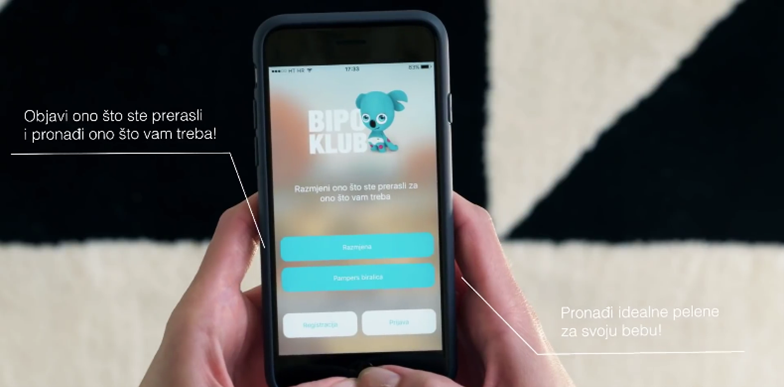
\includegraphics{Picture2.png}
			\caption{ Ulazak u aplikaciju, nudi dvije opcije Razmjenu i Pampers biralicu te registraciju i prijavu korisnika}
			\label{fig2}
		\end{figure}
		\newline
		\textit{Slično aplikaciji koja će nastati u ovom projektu, aplikacija je zatvorena na registrirane korisnike i na početnom zaslonu ima prijavu/registraciju korisnika. }\\
		\newline
		\textit{U aplikaciji koju razvijamo neregistrirani korisnik će se jedino moći registrirati u sustav na početnom zaslonu, a registrirani prijaviti. Nakon registracije korisniku stiže mail potvrde te se i on ima pravo prijaviti sada sa svojim korisničkim računom. Ulaskom u aplikaciju korisnik dalje može birati hoće li uređivati/pregledavati svoj profil i/ili dodavati podatke o djeci koji se koriste za filtriranje preporučenog sadržaja. Primjerice, korisnik ima muško dijete u dobi od 3 godine i ako na svom profilu doda podatke o dobi i spolu svog djeteta među preporučenim oglasima bit će samo predmeti za trogodišnjake.}\\
		\newline
		\begin{figure}[h!]
			\center
			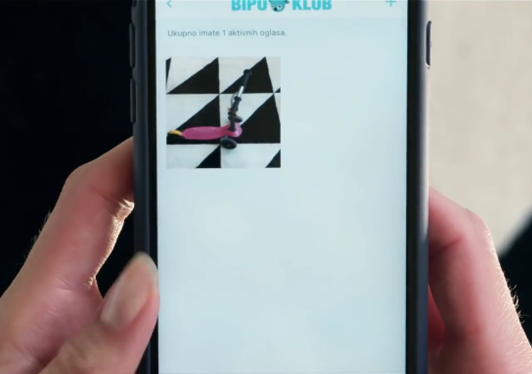
\includegraphics{Picture3.png}
			\caption{ Pregled aktivnih oglasa}
			\label{fig3}
		\end{figure}
		\newline
		\textit{Aplikacija omogućava korisniku pregled oglasa koje je postavio. Bit će implementirano i u našoj web aplikaciji. Naime, ako korisnik ima predmet koji želi donirati može to učiniti kreiranjem oglasa. Oglas se prije objave „šalje“ administratoru na pregled i ukoliko dobije zeleno svjetlo, oglas se objavljuje. Ako oglas slučajno nije valjan(nedostaju podaci ili su neispravni) administrator ga vraća korisniku na doradu, a ima i mogućnost odbiti oglas.}\\
		\newline
		\begin{figure}[h!]
			\center
			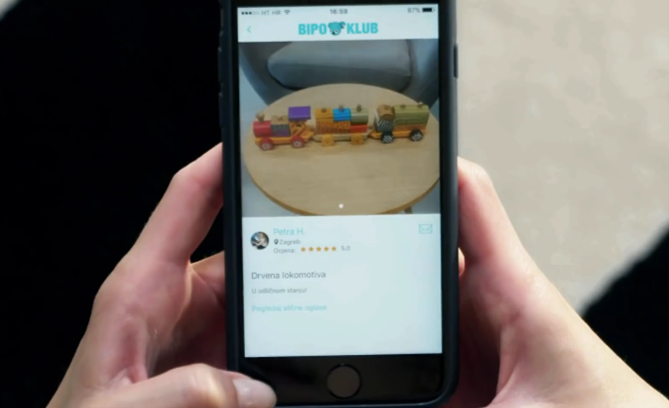
\includegraphics{Picture4.png}
			\caption{ Pregled tuđih oglasa}
			\label{fig4}
		\end{figure}
		\newline
		\textit{Aplikacija omogućava pregled postavljenih oglasa od strane drugih korisnika. Također, jedna od funkcionalnosti web aplikacije. }\\
		\newline
		\textit{Na temelju podataka koje je korisnik unio o djeci korisniku se prikazuju oglasi od najnovijih(do 3 dana starosti) prema najstarijima. Osim automatskog filtriranja koje rezultira preporučenim oglasima korisnik će moći i ručno postaviti dodatne filtere za oglase (odabrati kategorije). Uzmimo primjer od ranije da osoba ima muško dijete u dobi od 3 godine i zanimaju je igračke za sina. Tada će osoba dodatno postaviti filter, odnosno odabrati kategoriju dječjih igračaka, koje će ponovo biti filtrirane prema dobi i spolu(ako je definiran).   }\\
		\newline
		\begin{figure}[h!]
			\center
			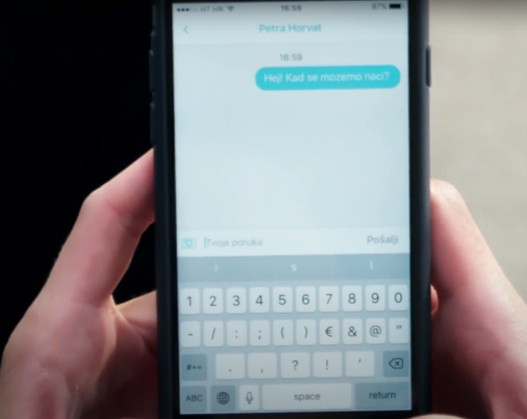
\includegraphics{Picture5.png}
			\caption{ Chat room sa donatorom}
			\label{fig5}
		\end{figure}
		\newline
		\textit{Aplikacija nudi direktno javljanje korisniku koji je postavio oglas kroz aplikaciju. Web aplikacija koja se razvija neće imati tu opciju te će se korisnici međusobno morati dogovarati van aplikacije.}\\
		\newline
		\textit{Po primitku donacije počinje odbrojavanje do trenutka kada će aplikacija ponuditi primatelju da isti predmet proslijedi dalje. Odbrojavanje se temelji na istraženim podacima o vremenu korištenja određenih predmeta. Primjerice, znamo da se kolica 3u1 koriste 1,5 godina i po isteku tog vremena korisniku koji je primio kolica u obliku donacije iskočit će prozor s upitom želi li možda proslijediti kolica dalje(donirati kreiranjem oglasa) ako su još u dobrom stanju.  }\\
		\newline
		\textit{Osim BIPO CLUB, mobilne aplikacije, postoje razne grupe na facebooku za razmjenu dječjih stvari (i prodaju) i odjeljak na njuškalu  „dječji svijet – sve za djecu i bebe“ koji nudi razmjenu i prodaju dječjih predmeta. }\\
		\newline
		\begin{figure}[h!]
			\center
			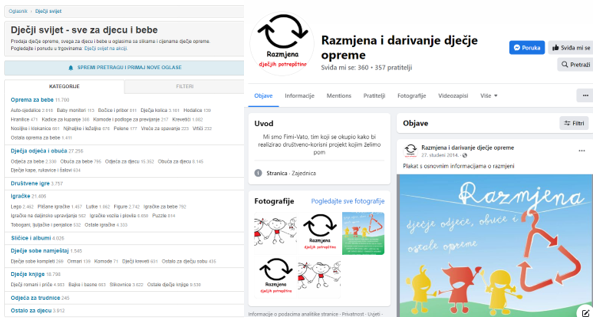
\includegraphics[width = \linewidth]{Picture6.png}
			\caption{Njuškalo (s lijeve strane) i facebook grupa (s desne strane)}
			\label{fig6}
		\end{figure}
		\newline
		\textit{Na kraju ovog projekta cilj je imati funkcionalnu web aplikaciju za doniranje i primanje predmeta putem oglasa. Kao što smo vidjeli istraživanje je pokazalo da ne postoje takve aplikacije i naša očekivanja su da bi aplikacija brzo postala popularna. }\\
		\newline
		\textit{Cijeli proces izrade počeo je analizom zahtjeva naručitelja, razradom funkcionalnih zahtjeva i izradom UML dijagrama(Use case dijagrama i sekvencijskih dijagrama) i ER modela baze podataka koja će čuvati sve podatke o korisnicima i pratiti oglase i razna dopuštenja. Rad se nastavlja programiranjem backenda i frontenda te obuhvaća pisanje popratne dokumentacije kao i testiranje same aplikacije u više faza i puštanje u pogon. Na kraju nas još očekuje prezentiranje same aplikacije i demonstracija implementiranih funkcionalnosti.}\\
		\newline
		\textit{Uvijek postoji mjesto za poboljšanje… Cijeli cilj ovog projekta je pomaganje zajednici tako da bi i nadogradnja aplikacije vodila ka stvaranju sigurnije i ravnopravne zajednice korisnika. }\\
		\newline
		\textit{Za veće zadovoljstvo korisnika i kako bi maksimizirali uspješnost doniranja i spajanja donatora sa korisnikom koji je prima sljedeća nadogradnja aplikacije bila bi usmjerena prema sustavu ocjenjivanja donatora i primatelja donacija (dvosmjerno ocjenjivanje) kao i sustavu za prijavljivanje korisnika koji krše opća pravila aplikacije i/ili sabotiraju uspješno doniranje predmeta. Nažalost, uvijek ima osoba koje žele iskoristiti druge ljude ili tuđu dobrotu. Kako bi smanjili mogućnost da jedan korisnik primi sve ili jako puno donacija u jako kratkom vremenu, ili nelogičnu kombinaciju donacija(prema podacima o djeci) i možda preproda iste predmete dok neki korisnici ostaju bez potrebnih predmeta uložili bi u razvijanje sustava za praćenje primljenih donacija.}\\
		\newline
		\textit{Cilj je imati što sigurniju zajednicu donatora i primatelja donacija te ulagati sustav za poticanje cirkuliranja predmeta i stalan priljev korisnika. }\\
		\newline
		\textit{Aplikacija bi omogućavala nadogradnje kao i prilagodbu na mobilne uređaje i tablete.}
		\eject
		